% \input{\pSections/"sec-case.tex"}

\section{PDES: Why}
%
\begin{frame}\frametitle{Relevance for SDA}
\begin{enumerate}
	\item Define \pdes
	\item Space domain application
	\item Parallelism challenges and opportunities
\end{enumerate}
\end{frame}

%     %     %     %     %     %     %     %     %
\subsection{PDES Fundamentals}
\begin{frame}\frametitle{Approaches}
	I am slide
\end{frame}

%     %     %     %     %     %     %     %     %
\subsection{Literature Survey}

\begin{frame}\frametitle{\href{https://www.cs.wm.edu/~andreas/}{\bl{Stathopoulos}}: \href{https://www.cs.wm.edu/~andreas/umsa/lectures/cs-sim-pdes.pdf}{Personal Web Page} \quad \mg{\scriptsize \raisebox{0.5ex}{\cite{Stathopoulos} \ \faUnlock}}}
\center
    % Hyperlink wraps around the image for clickable access
    \href{https://www.cs.wm.edu/~andreas/umsa/lectures/cs-sim-pdes.pdf}{
    \begin{overpic}[scale=0.325]
        % Main image (splash page or graphic)
        {\pLocalGraphics tombstones/Stathopoulos}
        % Add the unlocked symbol near the bottom-right of the image
        %\put(90,5){\faUnlock}
    \end{overpic}}
\end{frame}
%
\begin{frame}\frametitle{\href{https://www.cs.cmu.edu/~bryant/pubdir/MIT-LCS-TR-188.pdf}{\bl{Bryant}}: \href{https://publications.csail.mit.edu/lcs/pubs/pdf/MIT-LCS-TR-188.pdf}{Simulation of Packet Communication Architecture Systems} \quad \mg{\scriptsize \raisebox{0.5ex}{\cite{10.5555/889797} \ \faUnlock}}}
\center
	\href{https://apps.dtic.mil/sti/pdfs/ADA048290.pdf}{
	\begin{overpic}[ scale = 0.05 ]
		{\pLocalGraphics tombstones/pdes-alpha}
	\end{overpic}}
\end{frame}
%
\begin{frame}\frametitle{\bl{Chandy} \& \href{https://www.cs.utexas.edu/~misra/scannedPdf.dir/DistrSimulation.pdf}{\bl{Misra}: \href{https://publications.csail.mit.edu/lcs/pubs/pdf/MIT-LCS-TR-188.pdf}{Simulation of Packet Communication Architecture Systems} \quad \mg{\scriptsize \raisebox{0.5ex}{\cite{chandy1979distributed} \ \faUnlock}}}}
\center
	\href{https://ieeexplore.ieee.org/document/1702653}{
	\begin{overpic}[ scale = 0.125 ]
		{\pLocalGraphics tombstones/chandy-misra}
	\end{overpic}}
\end{frame}
%
\begin{frame}\frametitle{\href{https://faculty.cc.gatech.edu/~fujimoto/}{\bl{Fujimoto}}: Parallel discrete event simulation \quad \mg{\scriptsize \raisebox{0.5ex}{\cite{fujimoto1990parallel} \ \faUnlock}}}
\center
	\href{https://dl.acm.org/doi/10.1145/84537.84545}{
	\begin{overpic}[ scale = 0.05]
		{\pLocalGraphics tombstones/fujimoto-splash}
	\end{overpic}}
\end{frame}
%
\begin{frame}\frametitle{\href{https://scholar.google.com/citations?user=q1bkP7AAAAAJ}{Fujimoto} Citations: Military Engagements}
\center
\begin{enumerate}
	\item \fullcite{wieland1989performance}
	\item \fullcite{gilmer1988assessment}
\end{enumerate}
\end{frame}
%
\begin{frame}\frametitle{Other Citations: Military Engagements}
\center
\begin{enumerate}
	\item \fullcite{beckman1988distributed}
	\item \fullcite{gilmer1988assessment}
\end{enumerate}
\end{frame}
%
\begin{frame}\frametitle{\bl{Kunz}: Modeling and tools for network simulation \ \  \mg{\scriptsize \raisebox{0.5ex}{\cite{kunz2010parallel}}}}
\center
	\href{https://link.springer.com/chapter/10.1007/978-3-642-12331-3_8}{
	\begin{overpic}[ scale = 0.375]
		{\pLocalGraphics tombstones/kunz}
		\put(90,30) {\color{blue}\href{https://link.springer.com/book/10.1007/978-3-642-12331-3}{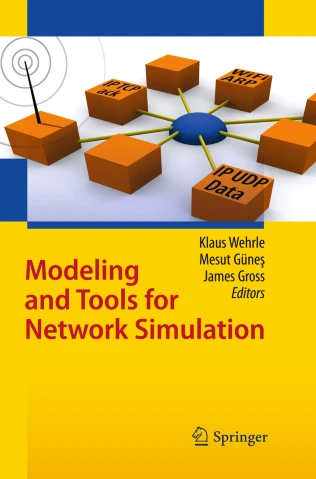
\includegraphics[ width = 1.5cm ]{\pLocalGraphics/978-3-642-12331-3}}}
	\end{overpic}}
\end{frame}

%\begin{frame}\frametitle{Stathopoulos: Personal Web Page \quad {\scriptsize{\mg{\cite{Stathopoulos}}} \,|\, \faUnlock}}
%\center
%	\href{https://www.cs.wm.edu/~andreas/umsa/lectures/cs-sim-pdes.pdf}{
%	\begin{overpic}[ scale = 0.325]
%		{\pLocalGraphics tombstones/Stathopoulos}
%		%\put(2,105) {\color{blue}{https://www.satobs.org/seesat/Aug-2010/0037.html}}
%	\end{overpic}}
%\end{frame}

%\begin{frame}\frametitle{Stathopoulos: Personal Web Page \quad {\scriptsize \raisebox{0.5ex}{\cite{Stathopoulos}} \, \tikz[baseline=-0.5ex]{\draw[thin] (0,0) -- (0,1.0em);} \, \raisebox{0.5ex}{\faUnlock}}}

%     %     %     %     %     %     %     %     %
\subsection{Tools for PDES}
\begin{frame}\frametitle{Experiment}
	I am slide
\end{frame}

\endinput  %  ==  ==  ==  ==  ==  ==  ==  ==  ==
